% final.tex
% Final Report for NM5660 Independent Study Module
% Author: Yih-Lun Huang
% Revisions: 16 April 2010

\documentclass{acm_proc_article-sp}

\usepackage{verbatim}
\usepackage{natbib}
\usepackage{url}

\hyphenation{trans-pa-ren-cy}

\begin{document}

% TODO: change to ``Toward...''?
\title{Investigation of the relationship between transparency and user
  experience}

\numberofauthors{1}
\author{
\alignauthor Yih-Lun Huang\\
\affaddr{HY090191Y}\\
\email{ylhuang@nus.edu.sg}
}

\maketitle
\begin{abstract}
[FIXME]
\end{abstract}


\category{H.5.2}{Information Interfaces And Presentation}{User
  Interface}[input devices and strategies]

\terms{Design, Algorithms, Measurement}

\keywords{Input device, multi-touch, touchpad, lazy}


\section{Introduction}
The notion of user experience has been wildly adopted in the field of
human-computer interaction. However, as many existing literature
pointed out already \citep{ux:hassenzahl, ux:law}, a common agreement
on the exact definition of user experience is still in debate, and is
so far not fully understood by the people---researchers, consultants,
managers in the industry, and practitioners---in the field.

They do agree that the traditional usability framework, which focus
primarily on user performance and user cognition, is limited and can
no longer model the ever more complex settings of the modern
computation. This was especially true when ubiquitous computing was
introduced, where the interfaces between users and computers are no
longer single, static, and restricted to the traditional window, icon,
menu, and pointing device. Instead, multiple interfaces are spread
through out the environment and are updated dynamically depending on
the context \citep{windows:bolter}.

But besides the above agreement, people from different backgrounds and
interests, with varying focuses and concerns, have formulated their
own definitions and statements on user experience. Some tackle from
the emotional and affective aspects of human-computer interaction,
such as stressing the importance of emotions as consequences of
product use. Some deal with the nature of experience or the
experiential aspect, e.g.\ \citet{experience:forlizzi}. And yet others
address the human needs beyond the instrumental, such as memories.

Though very exciting to witness and participate in this ``disordered''
time frame, where opportunities are still around to make significant
contributions to the human knowledge, it is actually quite troublesome
for practitioners in the field of human-computer interaction. And in
the case of this article, we specifically focus our attention on
software engineers.

\subsection{Patterns of User Experience}
Software engineers, like engineers in the other engineering
disciplines, rely on standards---codified and enforced from good
practices---to improve the quality and lower the cost of software
development \citep{practice:ipenz}. These standards can be in the form
of examples, guidelines or even abstractified into patterns. Patterns,
as described by \citet{patterns:griffiths}, are abstractions from the
specific examples, which give patterns their generative power. They do
not supply immediate solutions to the problems, however. Creativity is
required for the software engineers to implement the
patterns. Patterns are also considered more advantageous than
guidelines because they are more related to a context and are problem
centered \citep{patterns:welie}.

The traditional software patterns popularized by the `Gang of Four'
\citep{patterns:gamma} have shown tremendous importance to the
software development domain. They provide valuable engineering
solutions to difficult technical problems or elegant tricks to build
user interfaces. Mastering software patterns is so influential that it
is often regarded as an indication to distinguishing rockstar software
engineers from normal ones \citep{rockstar:iskold}.

Analogously, patterns of user experience---a language for describing
user experiences with structured information
\citep{pux:blackwell}---is the crucial factor for the success of bring
better user experience to the users. This is what practitioners like
software engineers want, instead of the exact definitions and
statements of user experience.

Interestingly, the traditional software patterns can also be
considered as patterns of user experience. But they are referring to
user experience for the \textit{software engineers}, i.e.\ software
engineers will have better experience with the source code if they
choose to implement appropriate software patterns into their
design. For example, following a well known software pattern can
increase the maintainability of the source code. Notice that this also
reflects an early, albeit still existing, common misconception of
software engineers \citep{pux:blackwell}. They often focus too much
attention on engineering the user interface and emphasizing the
technical details that, instead as supporting tools, these user
interface and technical details become the final product for the
users.

However the user experience we are mentioning here is the user
experience for the \textit{users}, the actual users who will be using
the software. By implementing these patterns of user experience into
the design, the users can gain better user experience with the
product. Table~\ref{tab:shield} gives a simple example on patterns of
user experience for error management \citep{patterns:welie}. Though
there are quite a few existing publications discussing patterns of
user experience in various aspects of human-computer interaction
(refer to section \ref{sec:relatedworks}), we will focus our attention
on investigating the patterns of user experience for interface
transparency.

\begin{table}[!t]
  \caption{Pattern of user experience `The Shield'.}
  \label{tab:shield}
  \begin{center}
    \begin{tabular}{| p{0.2\columnwidth} || p{0.7\columnwidth} |}
      \hline
      Name & The Shield. \\ \hline

      Problem & The user may accidentally select a function that has
      irreversible (side) effects. \\ \hline

      Usability Principle & Error management. \\ \hline

      Context & The user needs to be protected against unintended or
      accidental actions that have irreversible (side) effects. The
      (side) effects may lead to unsafe or highly undesired
      situations. For example the unintended deletion or overwriting
      of files. Do not use for actions that are reversible. \\ \hline

      Forces & The user is striving for speed while trying to avoid
      mistakes. \\ \hline

      Solutions & Protect the user by inserting a shield. \\ \hline

      Usability Impact & Increased safety, less errors and higher
      satisfaction. However, it requires extra user action which leads
      to lower performance time. \\ \hline

      Rationale & The extra layer causes the user to require 2
      repetitive mistakes instead of 1. The safe default decreases the
      chances for a second mistake. \\ \hline

      Known uses & Microsoft Explorer, Apple Finder. \\ \hline
    \end{tabular}
  \end{center}
\end{table}

\subsection{For Interface Transparency}
% Form pattern and guidelines for software engineer, with respect to
% interface transparency.
[Elaborated paragraphs explaining interface transparency as my second
  research interest.]

Added to this, the emergence of the user experience is an attempt to
inform design and evaluation has been widespread in HCI. Such that,
researchers are proposing user experience encapsulating the idea of
interface transparency.

Hence, the relationship between transparency and user
experience will also be examined.

\subsection{Research Goal}
[Elaborated paragraphs combining patterns of user experience and
  interface transparency as my research goal.]

% problem I am trying to solve
With all this being said, this article is not about yet another
attempt to develop a common view on user experience. Numerous
literature, conferences, and workshops have already attempted to
address this topic, such as \citet{early:forlizzi},
\citet{emotional:norman}, \citet{experience:forlizzi},
\citet{action:dourish}, \citet{ux:hassenzahl},
\citet{experience:desmet}, and \citet{ux:law}.

For sake of completeness, some view points on user experience will
still be discussed in the following section. However, the main
research goal for this article is to further explore interface
transparency within the field of user experience. Interface
transparency is still a crucial factor in this field, even though user
experience has been the prominent subject in recent years. In his
article, \citet{future:memmel} suggests that usability engineering and
interaction design will be the more concrete premises and disciplines
below the umbrella term of user experience. This complies with the
argument from \citet{windows:bolter} that transparency is only half
the story---each digital design should move back and forth between
being transparent and being reflective.

Transparent and reflective, two contrasting albeit interesting point
of views prompted people to think about whether they have been too
obsessed with achieving interface transparency, the benefits and
limitations of interface transparency, measuring interface
transparency. Added to this, the emergence of the user experience is
an attempt to inform design and evaluation has been widespread in
HCI. Such that, researchers are proposing user experience
encapsulating the idea of transparency. Hence, the relationship
between transparency and user experience will also be examined.

% Talk about the experiment.
\subsection{Experiment}
[FIXME]

A new human interface device and application will be developed to
investigate interface transparency within user experience. This new
device will provide similar functionality to the multi-touch touchpad
that comes with recent laptops. However, the device will enable the
users to perform the usual tasks of multi-touch touchpad on any
surface, as if the physical touchpad is underneath their hand. The
development of this new device is actually based upon our previous
study \citep{lmnt:huang}, where the first-generation prototype was
built and some preliminary studies were conducted. Much of the
feedback from the first-generation prototype are taken into
consideration when designing the new device for this study.

% Application based on Baba Painter.
An application will be developed to accompany the new human interface
device. This application will too be an extension to our other
previous study, an interactive painting and collaboration reviewing
system \citep{baba:abeyrathne}. However, since the instrument will be
replaced by the new device developed in this study, the scenario and
the users will be adjusted accordingly. We planed to target the
application to tots. The application will allow small children to
scrabble intuitively on any surface and be creative wherever they are,
whether on the dining table of a restaurant or on the wall in the
bedroom, meanwhile still avoid messing up the place.

% User, product, context

\subsection{Layout}
[Layout for the following sections.]


\section{Related Works}
\label{sec:relatedworks}
% TODO: mention Universal usability
[FIXME]

Many patterns of user experience from various facets of human-computer
interaction are also being published or discussed.  For instance,
\citet{patterns:tidwell} discussed about general subjects in
human-computer interaction; \citet{touch:boudreaux} talked exclusively
on user experience for multi-touch input device;
\citet{participatory:dearden} examined the patterns for enabling users
to participate in the product design.

\citet{unix:raymond}


\section{User Experience}
[FIXME]

When junior software engineers are given the task of designing a new
product or system\footnote{In the following text, ``product'' is used
  as a general term to refer to a product, system, service, or
  non-commercial item, unless explicitly specified otherwise.}, most
of the time, they tend to squeeze as many features as possible into
whatever they are suppose to design. The interfaces between the user
and the design are scattered all over. This can often be observed in
corporates where a junior software engineer is assigned to develop an
internal tool to facilitate an existing working process
(Figure~\ref{fig:featureful}.)  Though the design is practical, it is
not very useful and the usage is limited to only a small selected
group of users.

\begin{figure}[!t]
\centering
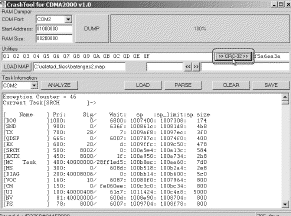
\includegraphics[width=.7\columnwidth]{featureful}
\caption{Internal tool for parsing the content in RAM.}
\label{fig:featureful}
\end{figure}

Software engineers have weird sense of excitement when they acquire
new technologies and are often very eager to try them out. Lack of
proper testing platform, many software engineers simply test the newly
acquired technology on whatever task they have at hand. Since efforts
and time are already spent on making the new technology functional and
it also provides a ``cool'' new feature to the original product, the
test is not removed afterward but instead becomes part of the product.

This is indicated by Alan Cooper \citeyearpar{inmates:cooper} that
although software engineers work hard to make their software easy to
use, their frame of reference is themselves and as a result they make
it easy for other software engineers, instead of normal users. He
explains that since having too much influence over the design of the
human interface and the lack of skills in this area, software
engineers do a poor job of it.

\subsection{Usability and Interface Transparency}
% TODO: talk about user-centered design and usability
This phenomenon will last until the software engineers are introduced
to the concept of usability. Dated back since the 1980s, this concept
was introduced by the published studies and analysis papers from a
dedicated group of mostly psychologists and human factors researchers
\citep{human:rubinstein, friendly:simpson, human:shneiderman,
  human:brown, software:dumas}. The philosophy behind this is that
every stage of the development process---requirements, design,
implementation, verification, and maintenance---are given great
attention to the needs and limitations of the users.

In this user-oriented development, contrast to the previous
technology-oriented or feature-oriented development, software
engineers work with experts from various specific fields---and most
importantly, also collaborate closely with the actual users---to bring
efficient, easy-to-learn, easy-to-memorize, and non-disruptive product
to the user. They form psychology and physiology model of the user to
anticipate their needs and limitations. And from that model, the
software engineers can build the product that would perfectly fit the
users.

% Bring up transparency, disrupt
From their field research, \citet{transparency:holtzblatt} show that
elements of an application design can disrupt users' work. They
observed that only when the users are not disrupted by the computer
system will they remain in the flow of their work and experience
interface transparency. This interface transparency is the ultimate
goal for usability studies and is considered as the ideal relationship
between user and tool with the tool seeming to disappear by
\citet{transparency:rutkoski}.

\subsection{Danger of Transparency}
% danger of transparency
However, the idea of striving for interface transparency is also
challenged by others. \citet{windows:bolter} talked about the myth of
transparency: \textit{The danger of transparency is that the interface
  will mask the operation of the system exactly when the user needs to
  see and understand what the system is doing}. As described by
\citet{design:norman}, the designers and the users each have their own
conceptual models or mental images of the product. Ideally, these two
models should be identical for the users to understand and use the
product properly. Unfortunately, this might not always be the case. So
the users often have to form their own model exclusively from the
observation of the product, whether from the exterior guise, the
feedback provided, the responses from blogger, documentations, and
etc. Therefore, if the product was invisible or transparent to the
users, how could it act as a medium to help the users to understand
itself? Nor can it be engaging or communicative.

% other direction: user experience
% difficulty of user experience
The community of human-computer interaction quickly embraced the
idea that solely pursuing for interface transparency and performance
is not enough, and a richer model is required to encapsulate the other
perspectives of the interaction, which fall under the umbrella term of
user experience. This may include addressing the human needs beyond
the instrumental; stressing affective and emotional aspects of the
interaction; and dealing with the nature of experience
\citep{ux:hassenzahl}. Many models have been proposed, however the
universal definition for user experience is still not well understood
nor fully clarified. There are several reasons why this is so,
according to the research from \citet{ux:law}:
\begin{enumerate}
  \item User experience is associated with a wide range of vague and
    dynamic concepts, including emotional, affective, experiential,
    hedonic, and aesthetic variables. Whether or not to include each
    of these variables is greatly dependent on the interests and
    background of the proposing author.
  \item The unit for measuring user experience is elastic. Unlike
    usability where only a single aspect of interaction between the
    user and the product\footnote{Just product, not including system
      nor service.} is assessed with well defined criteria, it could
    be extended to include multiple users, environment while the
    product is being used, and more.
\end{enumerate}


\section{Interface Transparency}
[FIXME]
% Talk about various other non interface transparency.

% Talk about Linux and Windows as example for transparency.


\section{Planned Experiment}
[FIXME]


\section{Conclusion}
[FIXME]


\bibliographystyle{apalike}
\bibliography{final}


\end{document}
